\documentclass[Main.tex]{subfiles} 
\begin{document}

%\subsection{Sprint 2}
%\begin{wrapfigure}{r}{0.6\textwidth}
%	\vspace{-20pt}
%    \centering
%	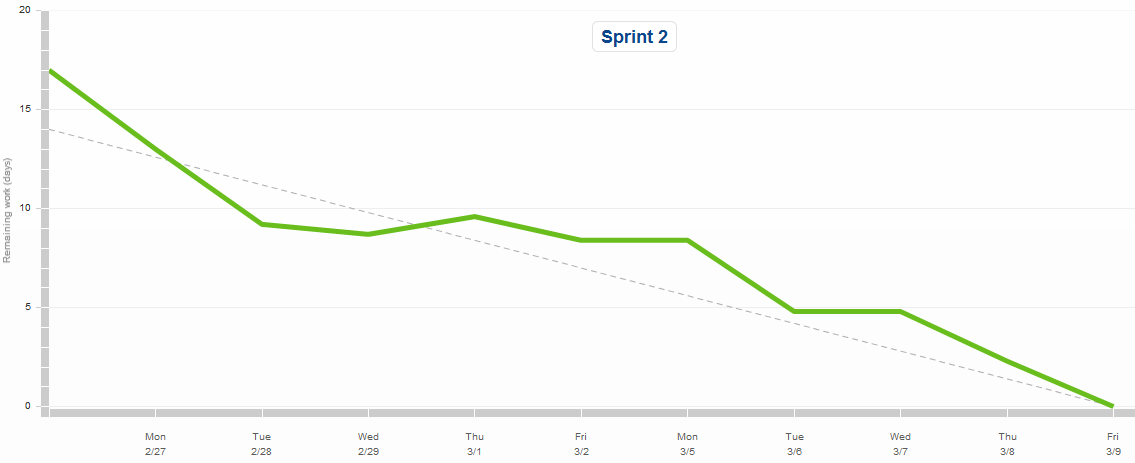
\includegraphics[scale=0.25]{Billeder/Sprint2_burn.png}
%	\vspace{-20pt}
%	\caption{Burndown chart for sprint 2}
%  \label{fig:sprint2}
%  \vspace{-10pt}
%\end{wrapfigure}
I sprint 2 blev databasen designet med tabeller og system sekvens diagrammer.
\\
Der blev ogs� �bnet op for de .dll-filer, som der skulle bruges til at tilg� robotten, og et simpelt program blev lavet, s� de forskellige funktioner kunne tilg�s. 
Yderligere dokumentation blev udformet til Use Case-diagrammet og Dom�nemodellen blev opdateret til, at passe med Use Case-diagrammet.
\\
\\
Kravspecifikationen blev ogs� opdateret og var t�t p� et f�rdigt stadie, hvorefter Systemarkitekturen blev p�begyndt.

\end{document}